% ______________________________________________________________________________
%
%   1DV600 - Software Technology
%   Assignment 2 -- "Analysis, Design and Implementation"
%
%  Author:  Jonas Sjöberg
%           Linnaeus University
%           js224eh@student.lnu.se
%           https://github.com/jonasjberg
%
%    Date:  2017-02-16 -- 2017-02-19
%
% License:  Creative Commons Attribution 4.0 International (CC BY 4.0)
%           <http://creativecommons.org/licenses/by/4.0/legalcode>
%           See LICENSE.md for additional licensing information.
% ______________________________________________________________________________


% ______________________________________________________________________________
\section{Task 2 -- Design}\label{task-2}

\paragraph{Instructions}\label{task-2-instructions}
from the course Wiki\cite{1dv600:lab2:instructions}:

\begin{quote}
  In this task you are to design the logic to fetch books in XML format (a
  suitable XML file is supplied). After reading the XML file it should be
  converted into objects in the running system and lastly translated into JSON
  for the web browser.
  Notice that this is a design task and therefore suitable design diagrams from
  UML are to be used to describe your solution (i.e. not code). You need to
  identify objects used in this and what messages they are sending, and when.
  As with the previous tasks, we also like you to write down your reflections
  in about 100 words.
\end{quote}


% ______________________________________________________________________________
\subsection{Design diagrams}\label{task-2-design}
The first design draft is shown in Figure~\ref{fig:uml-xmlrob} and
Figure~\ref{fig:uml-xmlseq}.

\begin{figure}[htbp]
  \centering
  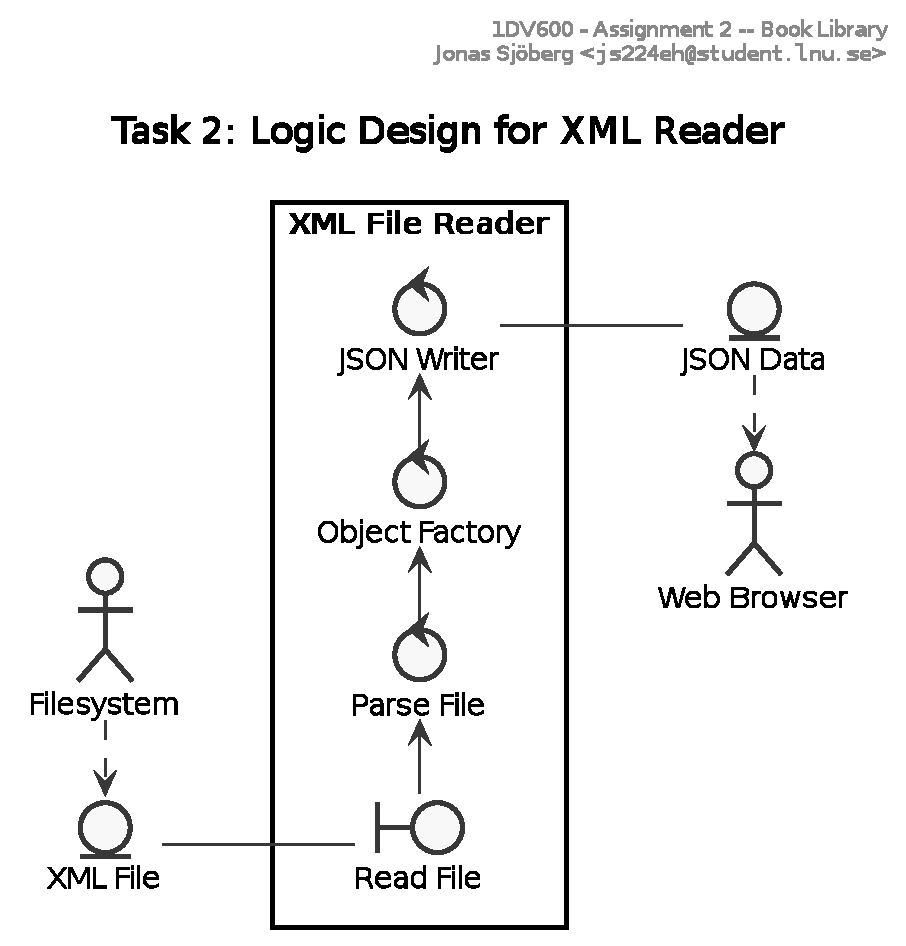
\includegraphics[width=0.75\linewidth]{include/uml-xml-design-rob.eps}
  \caption{UML Robustness Diagram for the XML File Reader}
  \label{fig:uml-xmlrob}
\end{figure}

\begin{figure}[htbp]
  \centering
  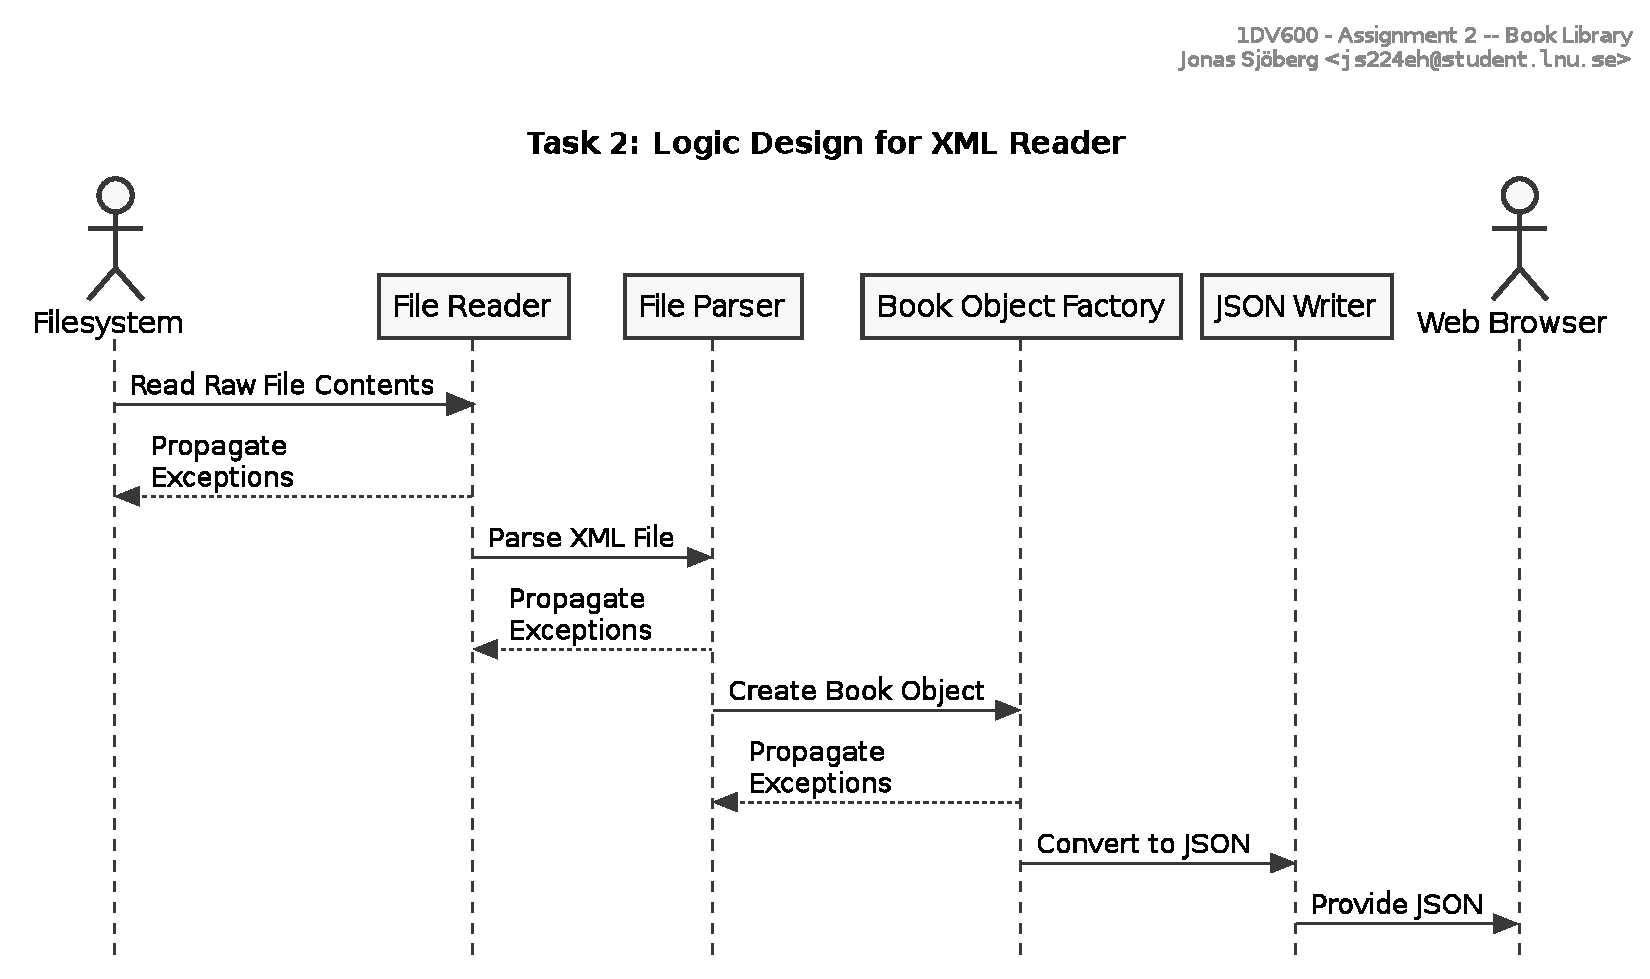
\includegraphics[width=1\linewidth]{include/uml-xml-design-seq.eps}
  \caption{UML Sequence Diagram for the XML File Reader}
  \label{fig:uml-xmlseq}
\end{figure}


It is not clear at this point how any exceptions, such as file read or
\texttt{XML} parsing errors should be handled. Exceptions should be propagated
from objects further down the call-chains, up to the user interface layer to be
displayed as some kind of warning message.



% ______________________________________________________________________________
\subsection{Reflections}\label{task-2-reflect}
Designing before coding is always wise, but my own personal style of reasoning
about how to solve programming problems does not necessarily line up with the
tools and frameworks provided by UML and its enclosing design-paradigm.

I also do not have enough insight or experience with the underlying framework
``dropwizard''\cite{framework:dropwizard} to make informed decisions on error
handling and logging, among other things.

